%======================================================================
% ANEXOS
%======================================================================
\chapter{Anexos}

\section{Anexo A: Glosario de Términos}

\begin{itemize}
    \item \textbf{AMD64}: Arquitectura de 64 bits
    \item \textbf{API}: Application Programming Interface
    \item \textbf{ASCII}: American Standard Code for Information Interchange
    \item \textbf{CLI}: Command Line Interface (Interfaz de Línea de Comandos)
    \item \textbf{ESB}: Enterprise Service Bus
    \item \textbf{gRPC}: Google Remote Procedure Call
    \item \textbf{HashMap}: Estructura de datos con búsqueda O(1)
    \item \textbf{JSON}: JavaScript Object Notation
    \item \textbf{NDJSON}: Newline Delimited JSON
    \item \textbf{O(1)}: Complejidad constante
    \item \textbf{O(n)}: Complejidad lineal
    \item \textbf{Protobuf}: Protocol Buffers
    \item \textbf{RAM}: Random Access Memory
    \item \textbf{RPC}: Remote Procedure Call
    \item \textbf{SIMD}: Single Instruction Multiple Data
    \item \textbf{SQL}: Structured Query Language
    \item \textbf{SSH}: Secure Shell
    \item \textbf{stdin}: Standard Input
    \item \textbf{stdout}: Standard Output
    \item \textbf{TLS}: Transport Layer Security
\end{itemize}

\section{Anexo B: Diagrama de Arquitectura de Flujo}

\begin{figure}[H]
    \centering
    \includegraphics[width=0.95\textwidth]{anexos/arquitectura_flujo.png}
    \caption{Diagrama de Arquitectura de Flujo}
    \label{fig:arquitectura-flujo}
\end{figure}

\section{Anexo C: Diagrama de Secuencia Principal}

\begin{figure}[H]
    \centering
    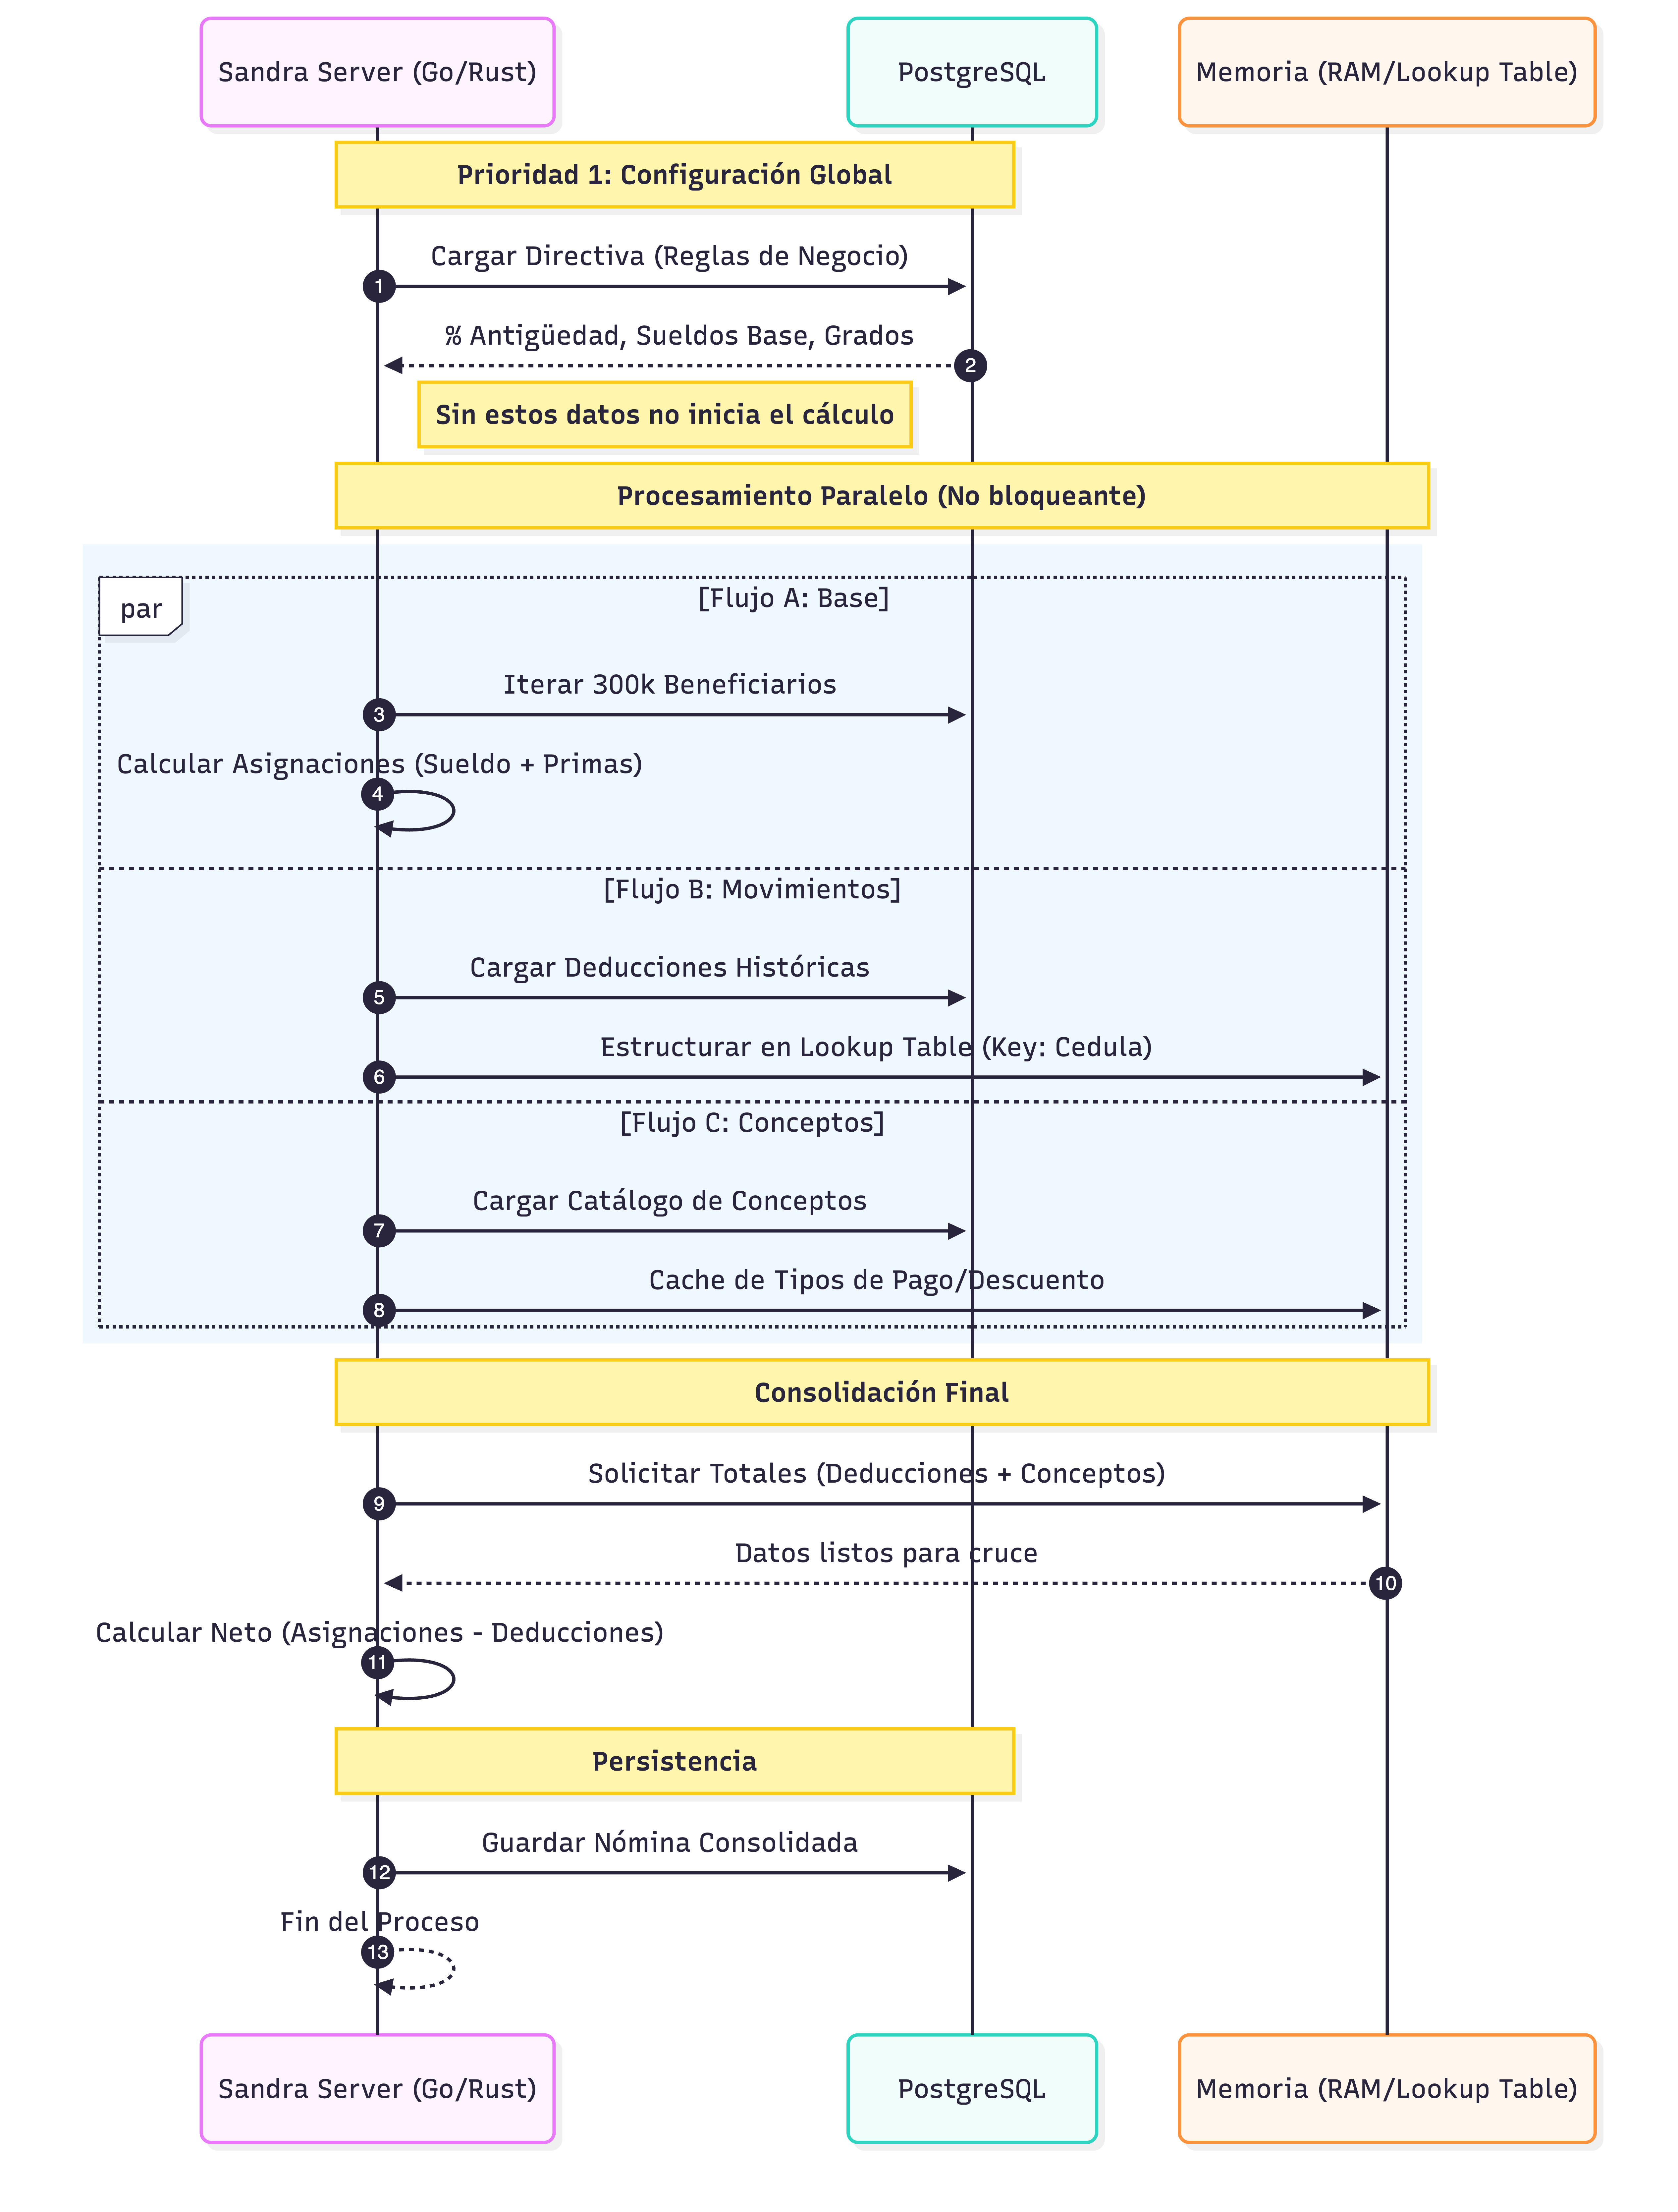
\includegraphics[width=0.95\textwidth]{anexos/secuencia_principal.png}
    \caption{Diagrama de Secuencia Principal}
    \label{fig:secuencia-principal}
\end{figure}

\section{Anexo D: Pipeline de Procesamiento}

\begin{figure}[H]
    \centering
    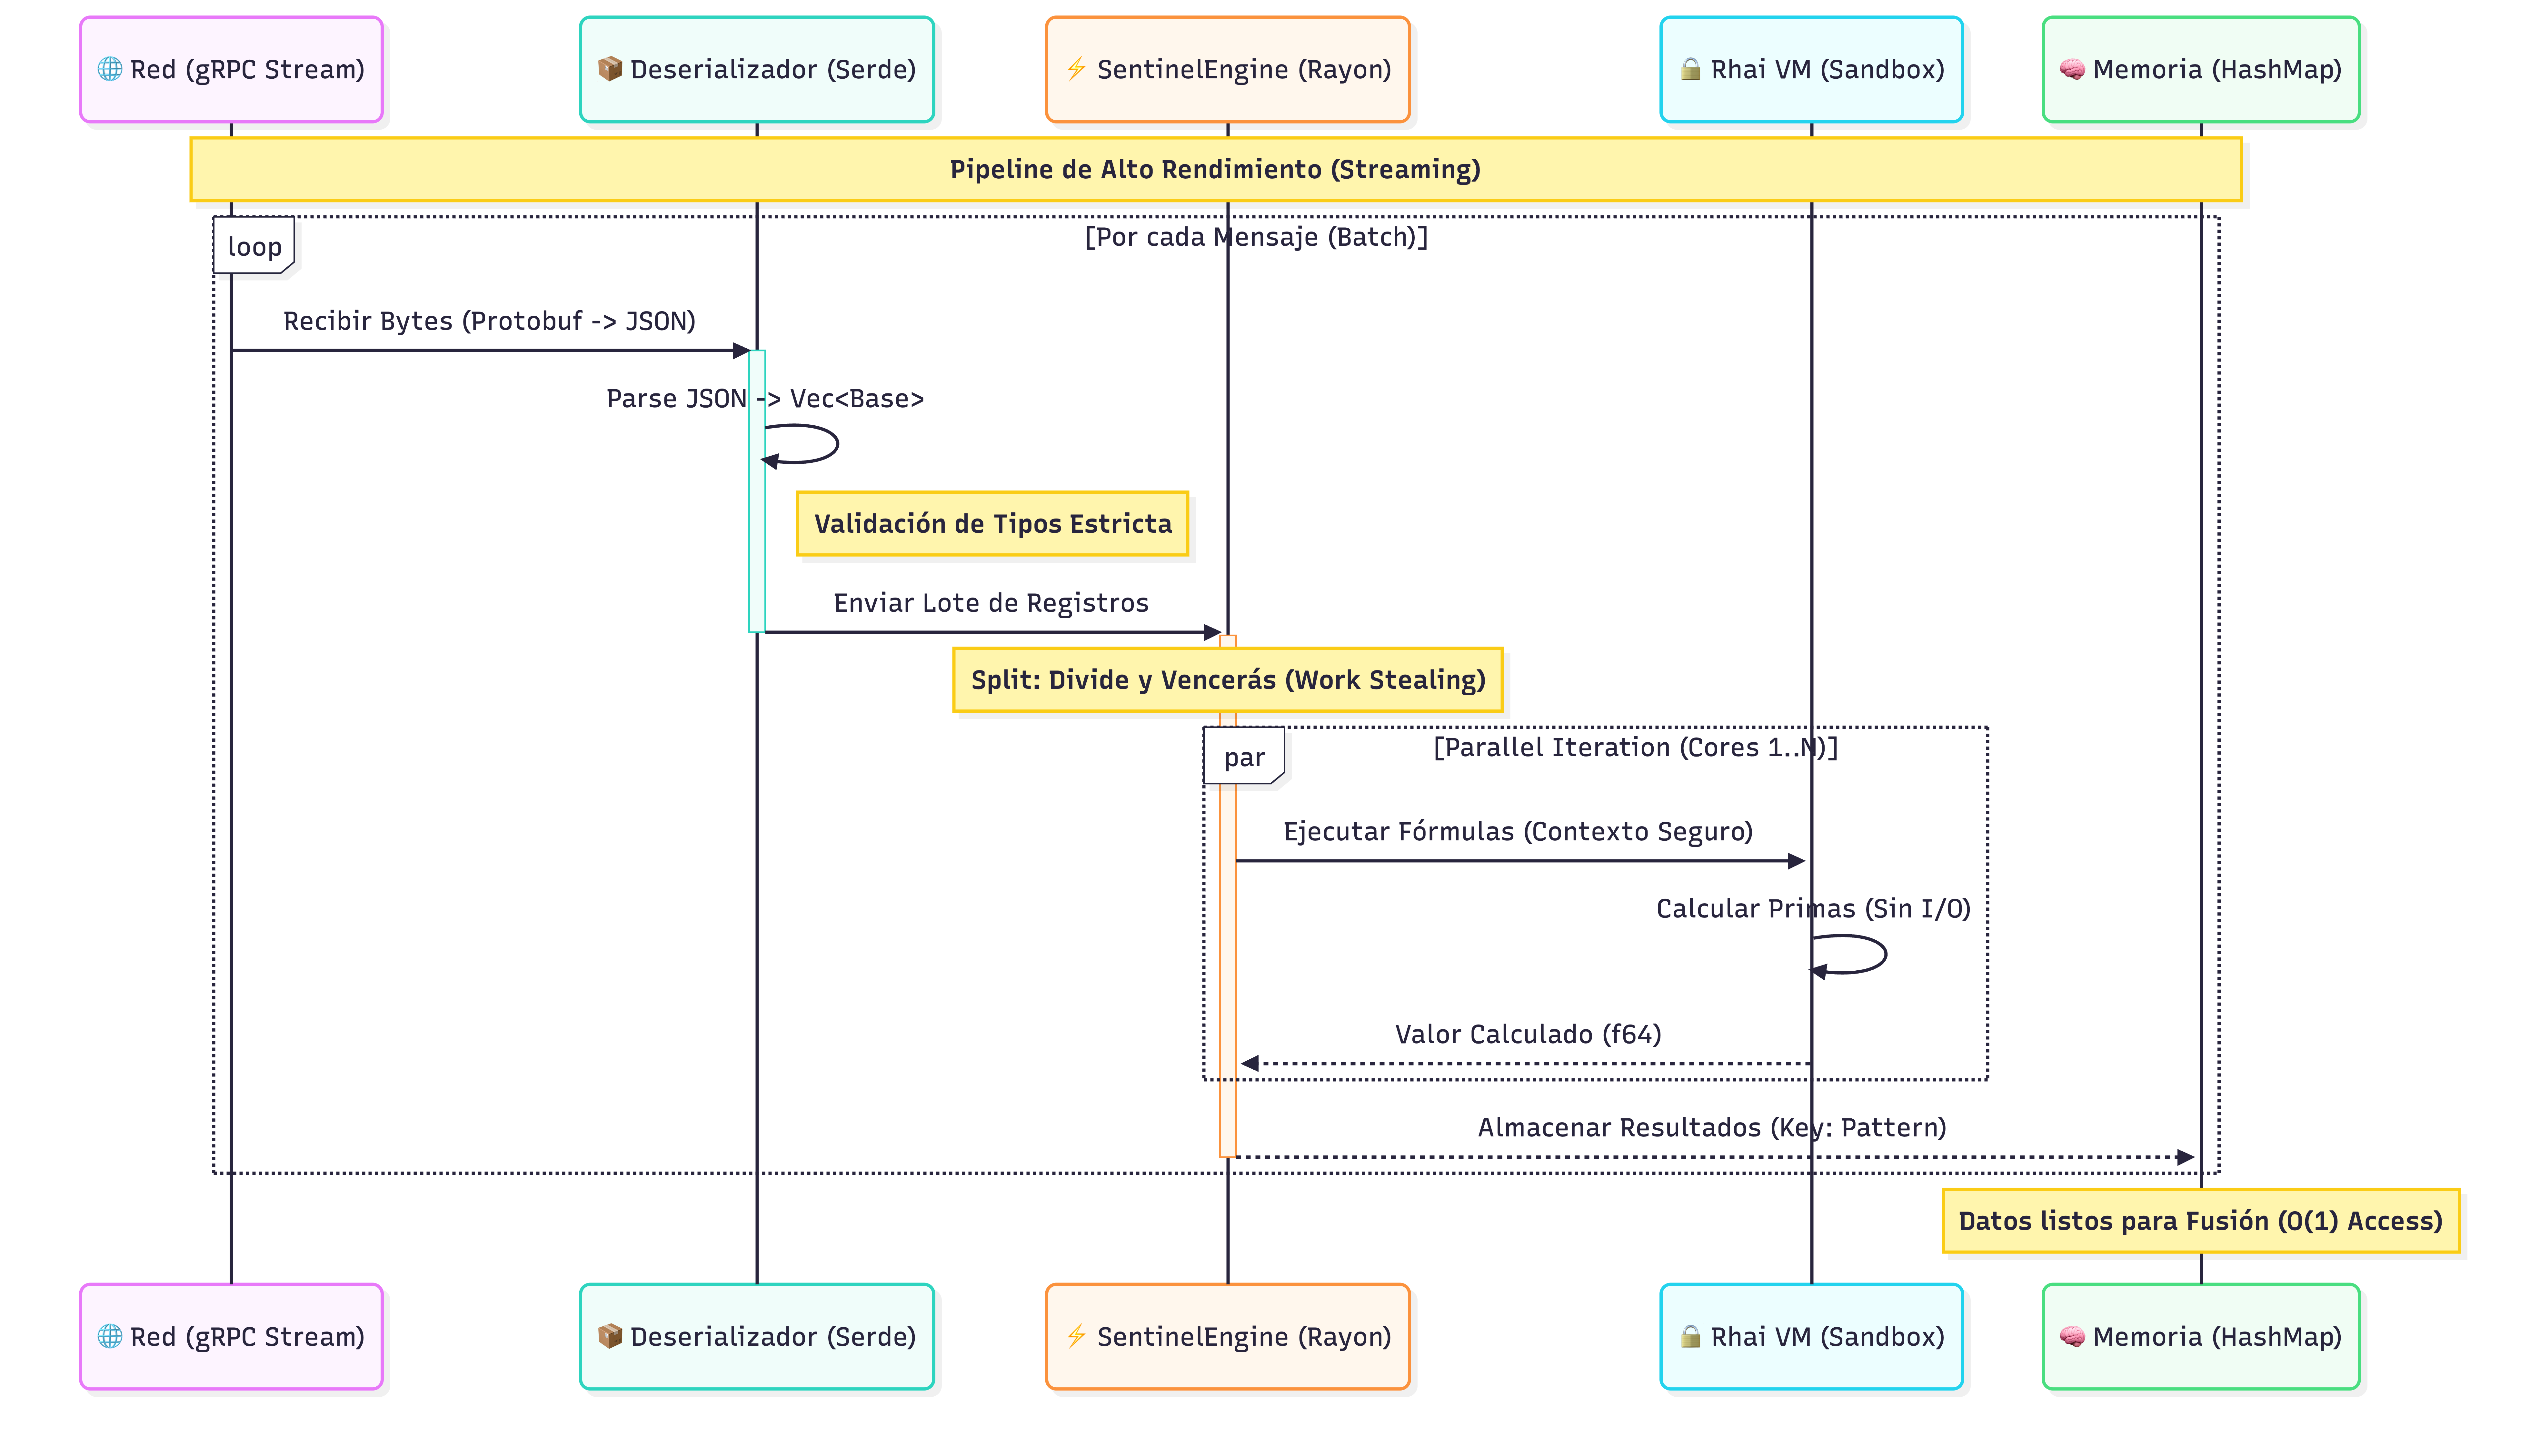
\includegraphics[width=0.95\textwidth]{anexos/pipeline_procesamiento.png}
    \caption{Pipeline de Alto Rendimiento}
    \label{fig:pipeline-procesamiento}
\end{figure}

\section{Anexo E: Formato de Archivos de Exportación}

\subsection{E.1 Formato nomina exportada.csv}

\begin{center}
\begin{tabular}{lp{10cm}}
\toprule
Campo & Descripción \\
\midrule
cedula & Identificador único del beneficiario \\
nombres & Nombres del trabajador \\
apellidos & Apellidos del trabajador \\
sexo & Sexo del trabajador \\
edo civil & Estado civil \\
n hijos & Número de hijos \\
componente id & Identificador del componente \\
grado id & Identificador del grado \\
... & (campos adicionales según configuración) \\
\bottomrule
\end{tabular}
\end{center}

\subsection{E.2 Formato aporte CICLO.csv}

\begin{center}
\begin{tabular}{lp{10cm}}
\toprule
Campo & Descripción \\
\midrule
cedula & Identificador único del beneficiario \\
nombres & Nombres del trabajador \\
apellidos & Apellidos del trabajador \\
numero cuenta & Número de cuenta bancaria \\
garantia original & Garantía calculada original \\
factor aplicado & Factor de proporción aplicado \\
garantia anticipo & Garantía distribuida (anticipo) \\
\bottomrule
\end{tabular}
\end{center}

\newpage
